\chapter{One-dimensional trapped spinless fermions}\label{ch:fermion_1d}

We now investigate a series of results for the one-dimensional trapped spinless fermions with Gaussian interaction. Here, all fermions are constrained to have spin in the same polarisation. A better description of the physics of the problem is given in \ref{sec:choice_of_systems}.

\section{Initial Comparisons}

We begin by demonstrating in \figref{fig:E_conv_ferm_pol_NI} that all three main trial wavefunctions discussed in \secref{sec:ansatz_closer_view} can very quickly converge to yield the ground-state of the non-interactive system. This serves as a valuable reference point for the code. These results were obtained without any hyperparameter search or addition of a correlation factor, showing that it is a fairly easy result to obtain. In these experiments, we used the Adam optimiser with learning rate $\alpha = 0.01 * c$ for all models, where $c$ is a scaling factor used both for the Metropolis step and for the learning rates, and equates to $1/\sqrt{N\cdot d}$. All results hereafter will use a Metropolis step of $0.1/\sqrt{N\cdot d}$ as this was shown to be optimal.
\begin{figure}[H]
    \centering
    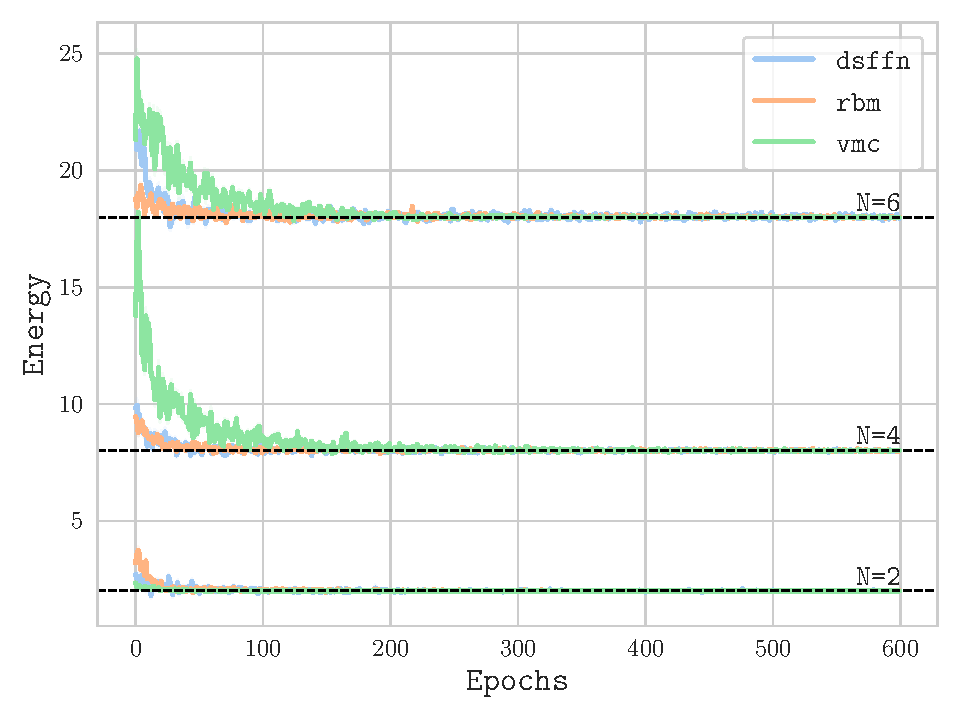
\includegraphics[width=0.55\linewidth]{Chapters/Results/N2/E_conv_ferm_pol_NI.pdf}
    \caption{Energy convergence curve for the non-interactive one-dimensional fully polarised fermionic system. In black dotted line, the analytical ground-state energies are marked. The models are Deep Set feed-forward network (DSFFN), restricted Boltzmann machine (RBM) and a standard variational Monte Carlo (VMC). Here we used Adam with learning rate of $0.01$ and Metropolis sampling.}
    \label{fig:E_conv_ferm_pol_NI}
\end{figure}

To check if reaching the ground-state energy results in an accurate wavefunction representation, one can generate a plot of the wavefunction. This is especially possible in the one-dimensional two-particle scenario, where the positions of each particle can be used as axes and the function value can be represented by a colorbar, as in \figref{fig:1D2P}. The values were obtained by uniformly sampling the positions for the particles and evaluating the output of a trained model, together with its sign. \figref{fig:1D2P} further serves to validate that despite working with $\ln|\psi|$ throughout the entire sampling and training process, we can recover the sign of the wavefunction. The profile shown is a classic fermionic representation, with a node region at $X_1 = X_2$ around which the wavefunction values are mirrored, except for a flip in sign. This is a consequence of the Pauli exclusion principle and the fact that we enforce the fermions to be polarised with the same spin.

\begin{figure}[H]
    \centering
    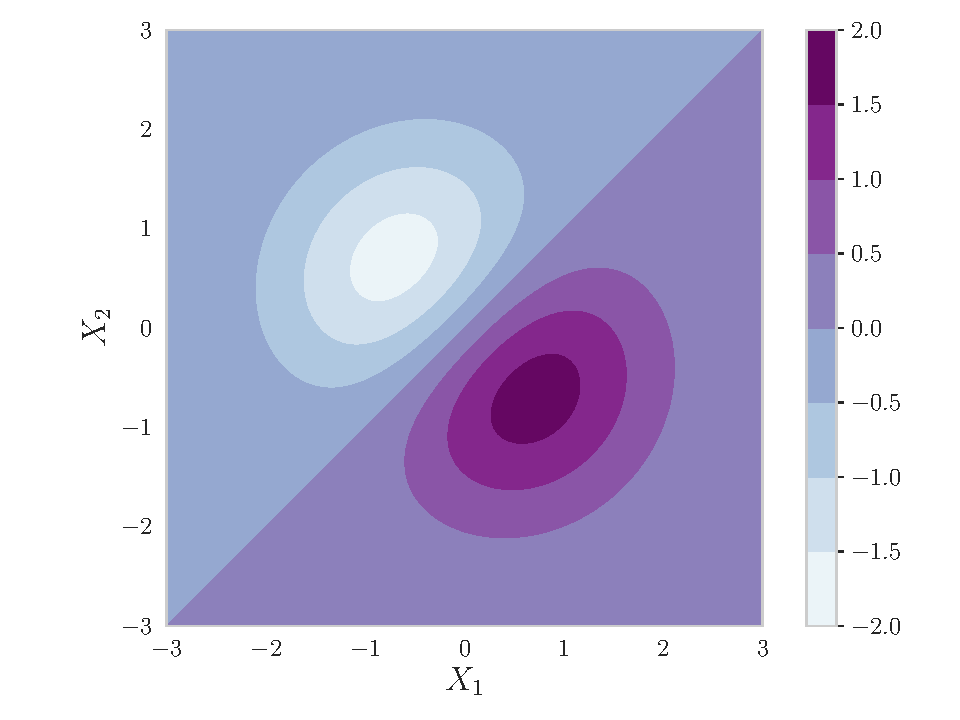
\includegraphics[width=0.7\linewidth]{Chapters/Results/N2/1D2P_wave_function.pdf}
    \caption{Two particle wavefunction for a one-dimensional fermionic ground-state. A clear fermionic nodal structure at $X_1 = X_2$ can be observed.}
    \label{fig:1D2P}
\end{figure}

We can compare the quality of our models and techniques without extensive parameter investigation for a small but interacting system of two particles ($N = 2$). At this stage, the results shown are merely investigations and are not fine-tuned in any way. In \figref{fig:N2_models_differentV0}, we compare our models with four values of interaction strength. We begin with an attractive regime of $V_0 = - 20$ and increase until we obtain a repulsive interaction $V_0 = 20$. In all interactive polarised fermionic systems, we limit ourselves to dealing with an interaction range of $\sigma_0 = 0.5$. The energy values displayed are a rolling average over ten epochs for better visuals. If, for example, 600 epochs were used, only 60 points make up the plot. 

Furthermore, \figref{fig:N2_models_differentV0} contains Hartree-Fock and CI energies, obtained with the code available from \cite{drissifermion}. It should be mentioned that the basis for the CI calculations was by no means a large one, with only 20 harmonic oscillator modes, and the Hartree-Fock calculations were obtained via $N$ integro-differential equations, where we iterate over the entire spatial grid computing the density and updating the Hamiltonian matrix at each step. Then, approximate eigenvalues are obtained via the Rayleigh-Ritz method.

All results shown in \figref{fig:N2_models_differentV0} used a block-diagonal approximation of the stochastic reconfiguration (SR) update rule with learning rate of $10^{-3}$. For all uses of this SR approximation, we also added a diagonal shift of $\lambda = 10^{-4}$ and a trust region for the update, described in \secref{sec:kfac}. The convergence curves have large deviations because small batch sizes were used. This means that only 500 MC proposals were sampled to collect the averages at each step. Consequently, the energy estimations fluctuate, and the gradient update, which is based on $\nabla \langle E_L\rangle$, also loses stability. 
\begin{figure}[H]
    \centering
    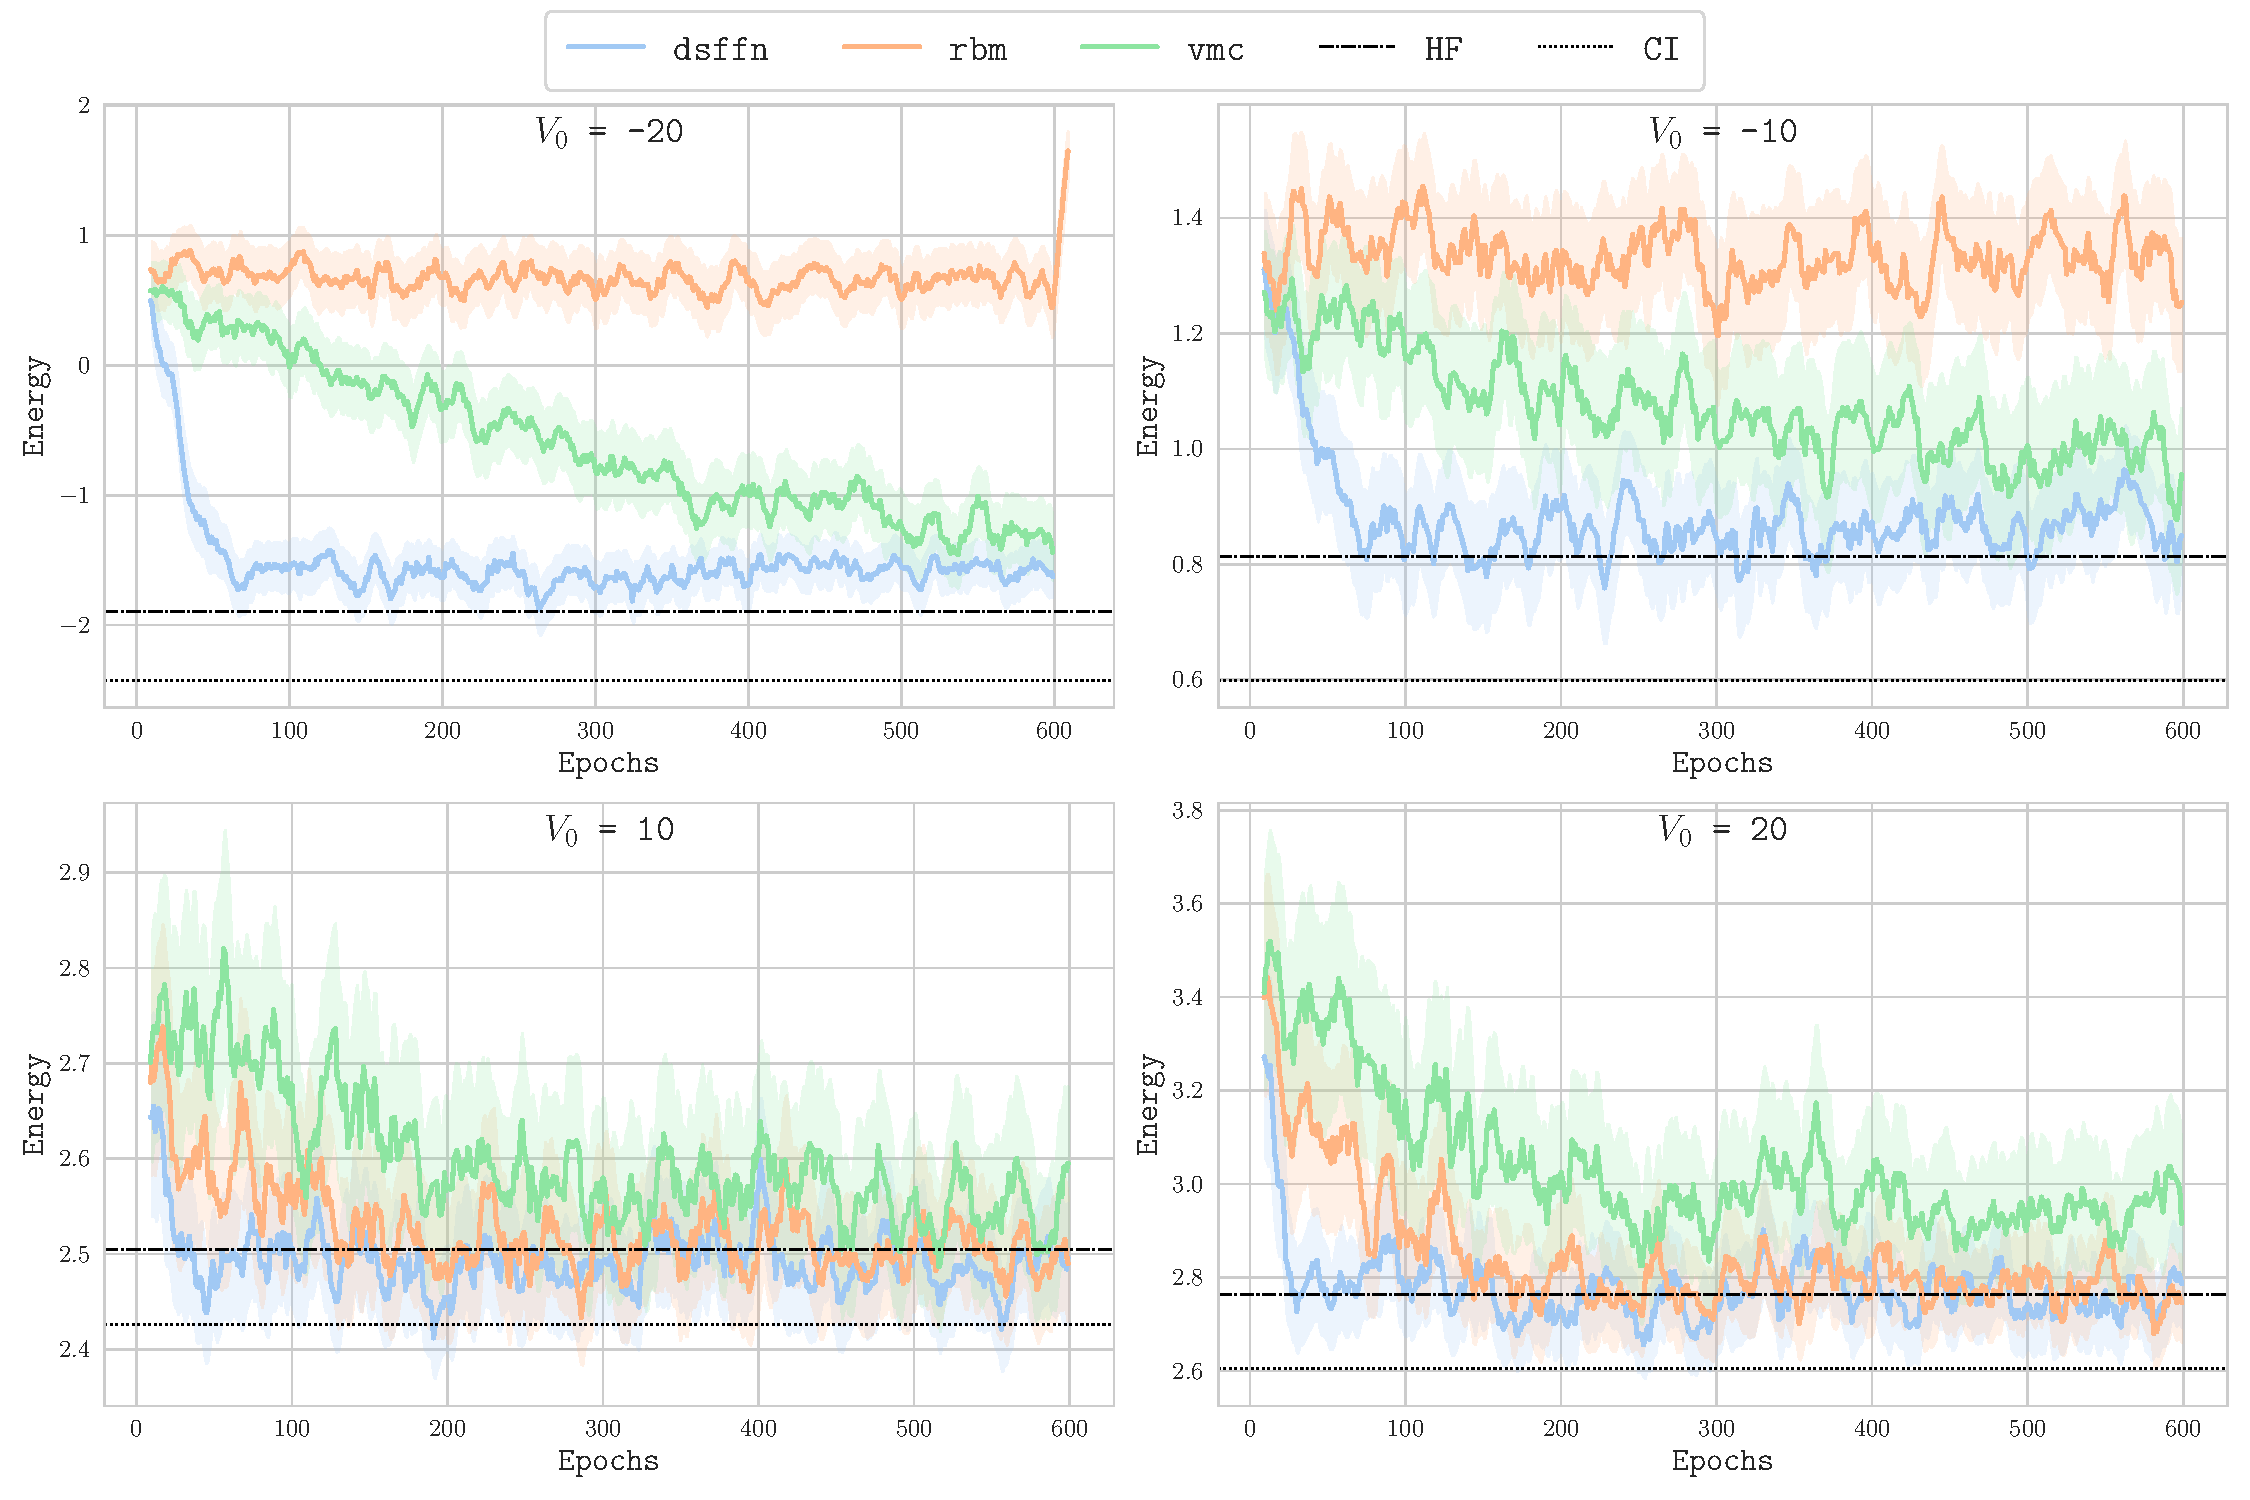
\includegraphics[width=1\linewidth]{Chapters/Results/N2/energy_convergence_v0_all.pdf}
    \caption{Energy convergence curve for the two particle ($N=2$) interactive problem of one-dimensional fully polarised fermions. The shaded area marks a $95\%$ confidence interval. In black dotted line, one can see Hartree-Fock and CI reference energies. None of the models used were fine-tuned, and the optimiser sheme was the stochastic reconfiguration method with a block-diagonal approximation.}
    \label{fig:N2_models_differentV0}
\end{figure}

Still with regard to \figref{fig:N2_models_differentV0}, the Deep Set model seems to outperform the other two, especially in the attractive regime. Although this could be attributed to a larger expressive power or more careful enforcement of \as, special mention must be credited to the pretraining stage. As detailed in \secref{sec:pretrain}, for feedforward networks, convergence for dimensions greater than one was only achieved by pre-training the ansatz in a supervised manner. Specifically, we fit the log probability of the ansatz to that of a multivariate Gaussian. It is known that in the attractive regime, the one-dimensional spinless fermions exhibit a density profile similar to non-interacting bosons \cite{valiente2020bose}, resulting in a density profile that closely resembles a Gaussian. This, together with a larger and expressive power and flexibility, can explain why the DSFFN performs better than the other models in the attractive regime.

\subsection{Correlation Factor}

A last analysis without extensive parameter experimentation can be seen in \figref{fig:jastrow}, where we select the deep set FFN ansatz of figure \figref{fig:N2_models_differentV0} for the same physical systems and compare convergence curves with and without the inclusion of the Jastrow factor. We see that, without the Jastrow factor, the model is capable of oscillating around the energy levels given by the Hartree-Fock calculations. Indeed, this variational ansatz uses a Gaussian envelope only with the determinant of Hermite polynomials, then approximating a single Slater determinant. Only with the introduction of the Jastrow factor can the energy values achieved go significantly lower than the HF approximation.

This observation is interesting. In principle, the universal approximation theorem guarantees that the neural network part of the ansatz can approximate any complex correlation factor which is not captured by the HF approximation. Although this might indeed be possible, the explicit addition of a correlation factor to the ansatz was what significantly enabled energies lower than HF. However, the statistics in \figref{fig:jastrow} are lacking, and we must examine the values and errors of larger Monte Carlo samples to be able to make this affirmation.

\begin{figure}[H]
    \centering
    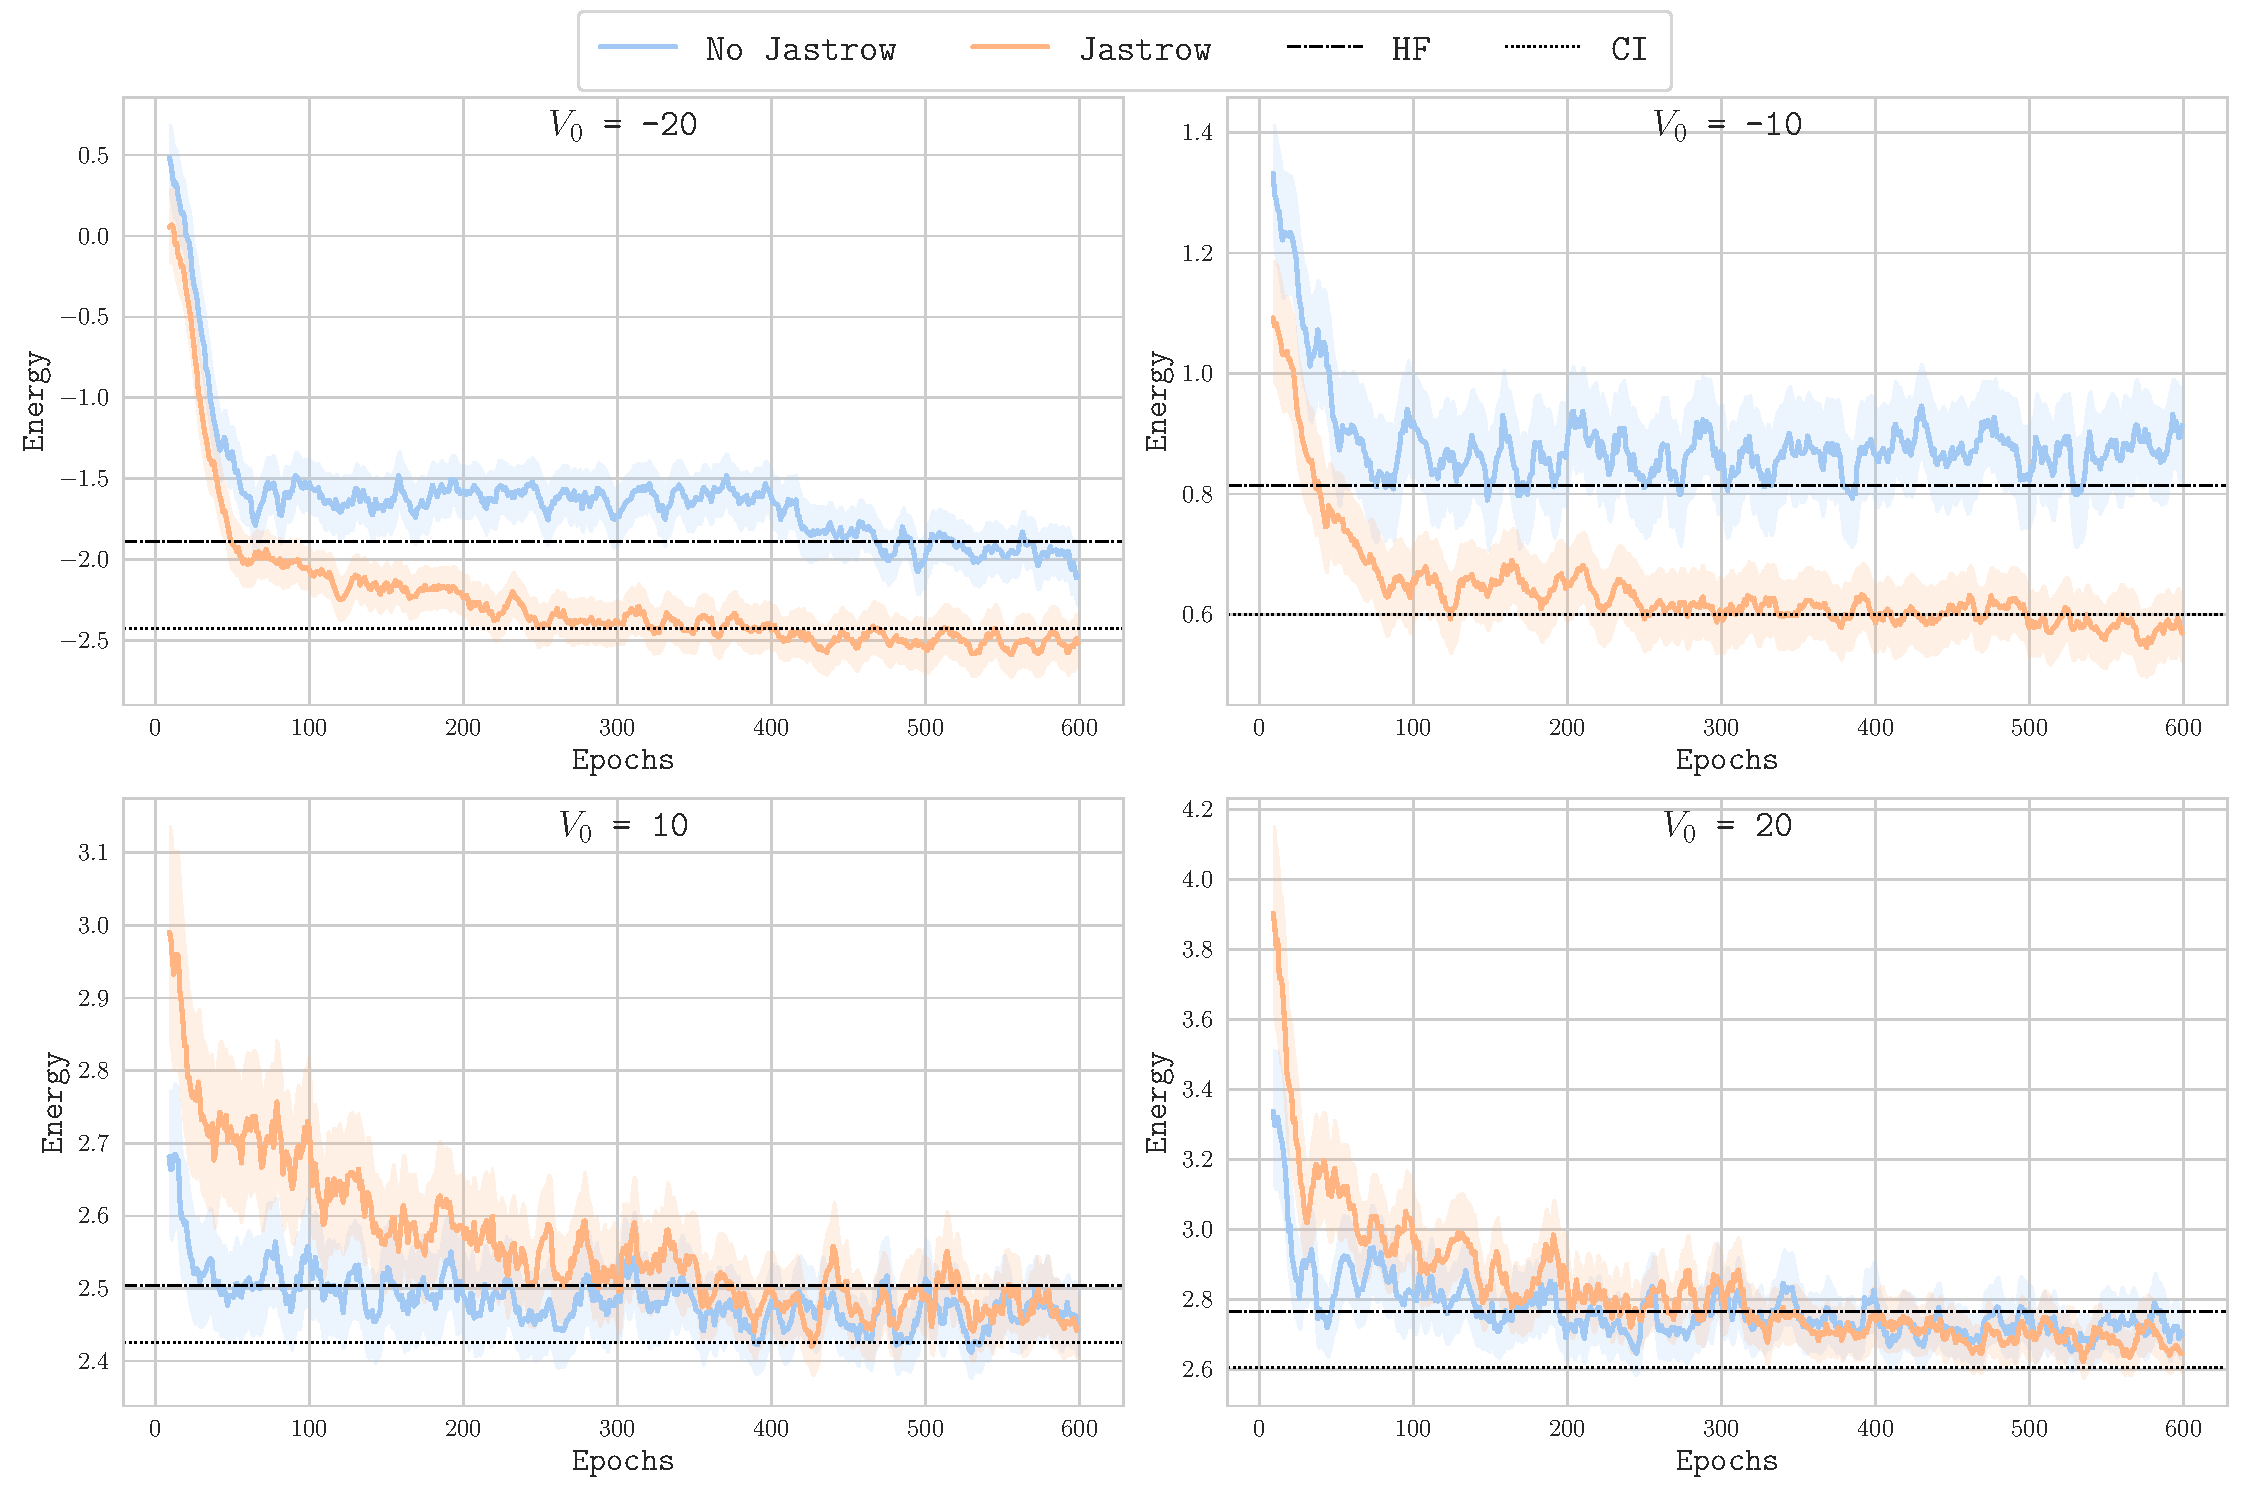
\includegraphics[width=1\linewidth]{Chapters/Results/N2/dsffnn_jastrow_energy_convergence_v0_all.pdf}
    \caption{Comparison between energy convergence curves for two particle ($N = 2$) for Deep Set feed-forward network with and without Jastrow factor. We an approximate stochastic reconfiguration optimiser, and the plot is displayer with a running average of 10 epochs. The shaded are represents a $95\%$ confidence interval.}
    \label{fig:jastrow}
\end{figure}

\section{Hyperparameter Search}\label{sec:sweep1d}

We then proceed to more thorough investigations via hyperparameter sweep searches. For each of our ansatz, we performed a sweep of approximately 300 configurations. This means that 300 sets of variational training were done, each with a random combination of options such as batch size, learning rate (here called ``Eta''), maximum training epochs, network architecture, and more. Figure \ref{fig:ds_complete_sweep} displays the sweep for the Deep Set ansatz, which involved 351 hyperparameter configurations. Analogous searches for VMC and RBM ansätze can be seen in the appendix \ref{apendix:more_results_1d}.

\begin{figure}[H]
    \centering
    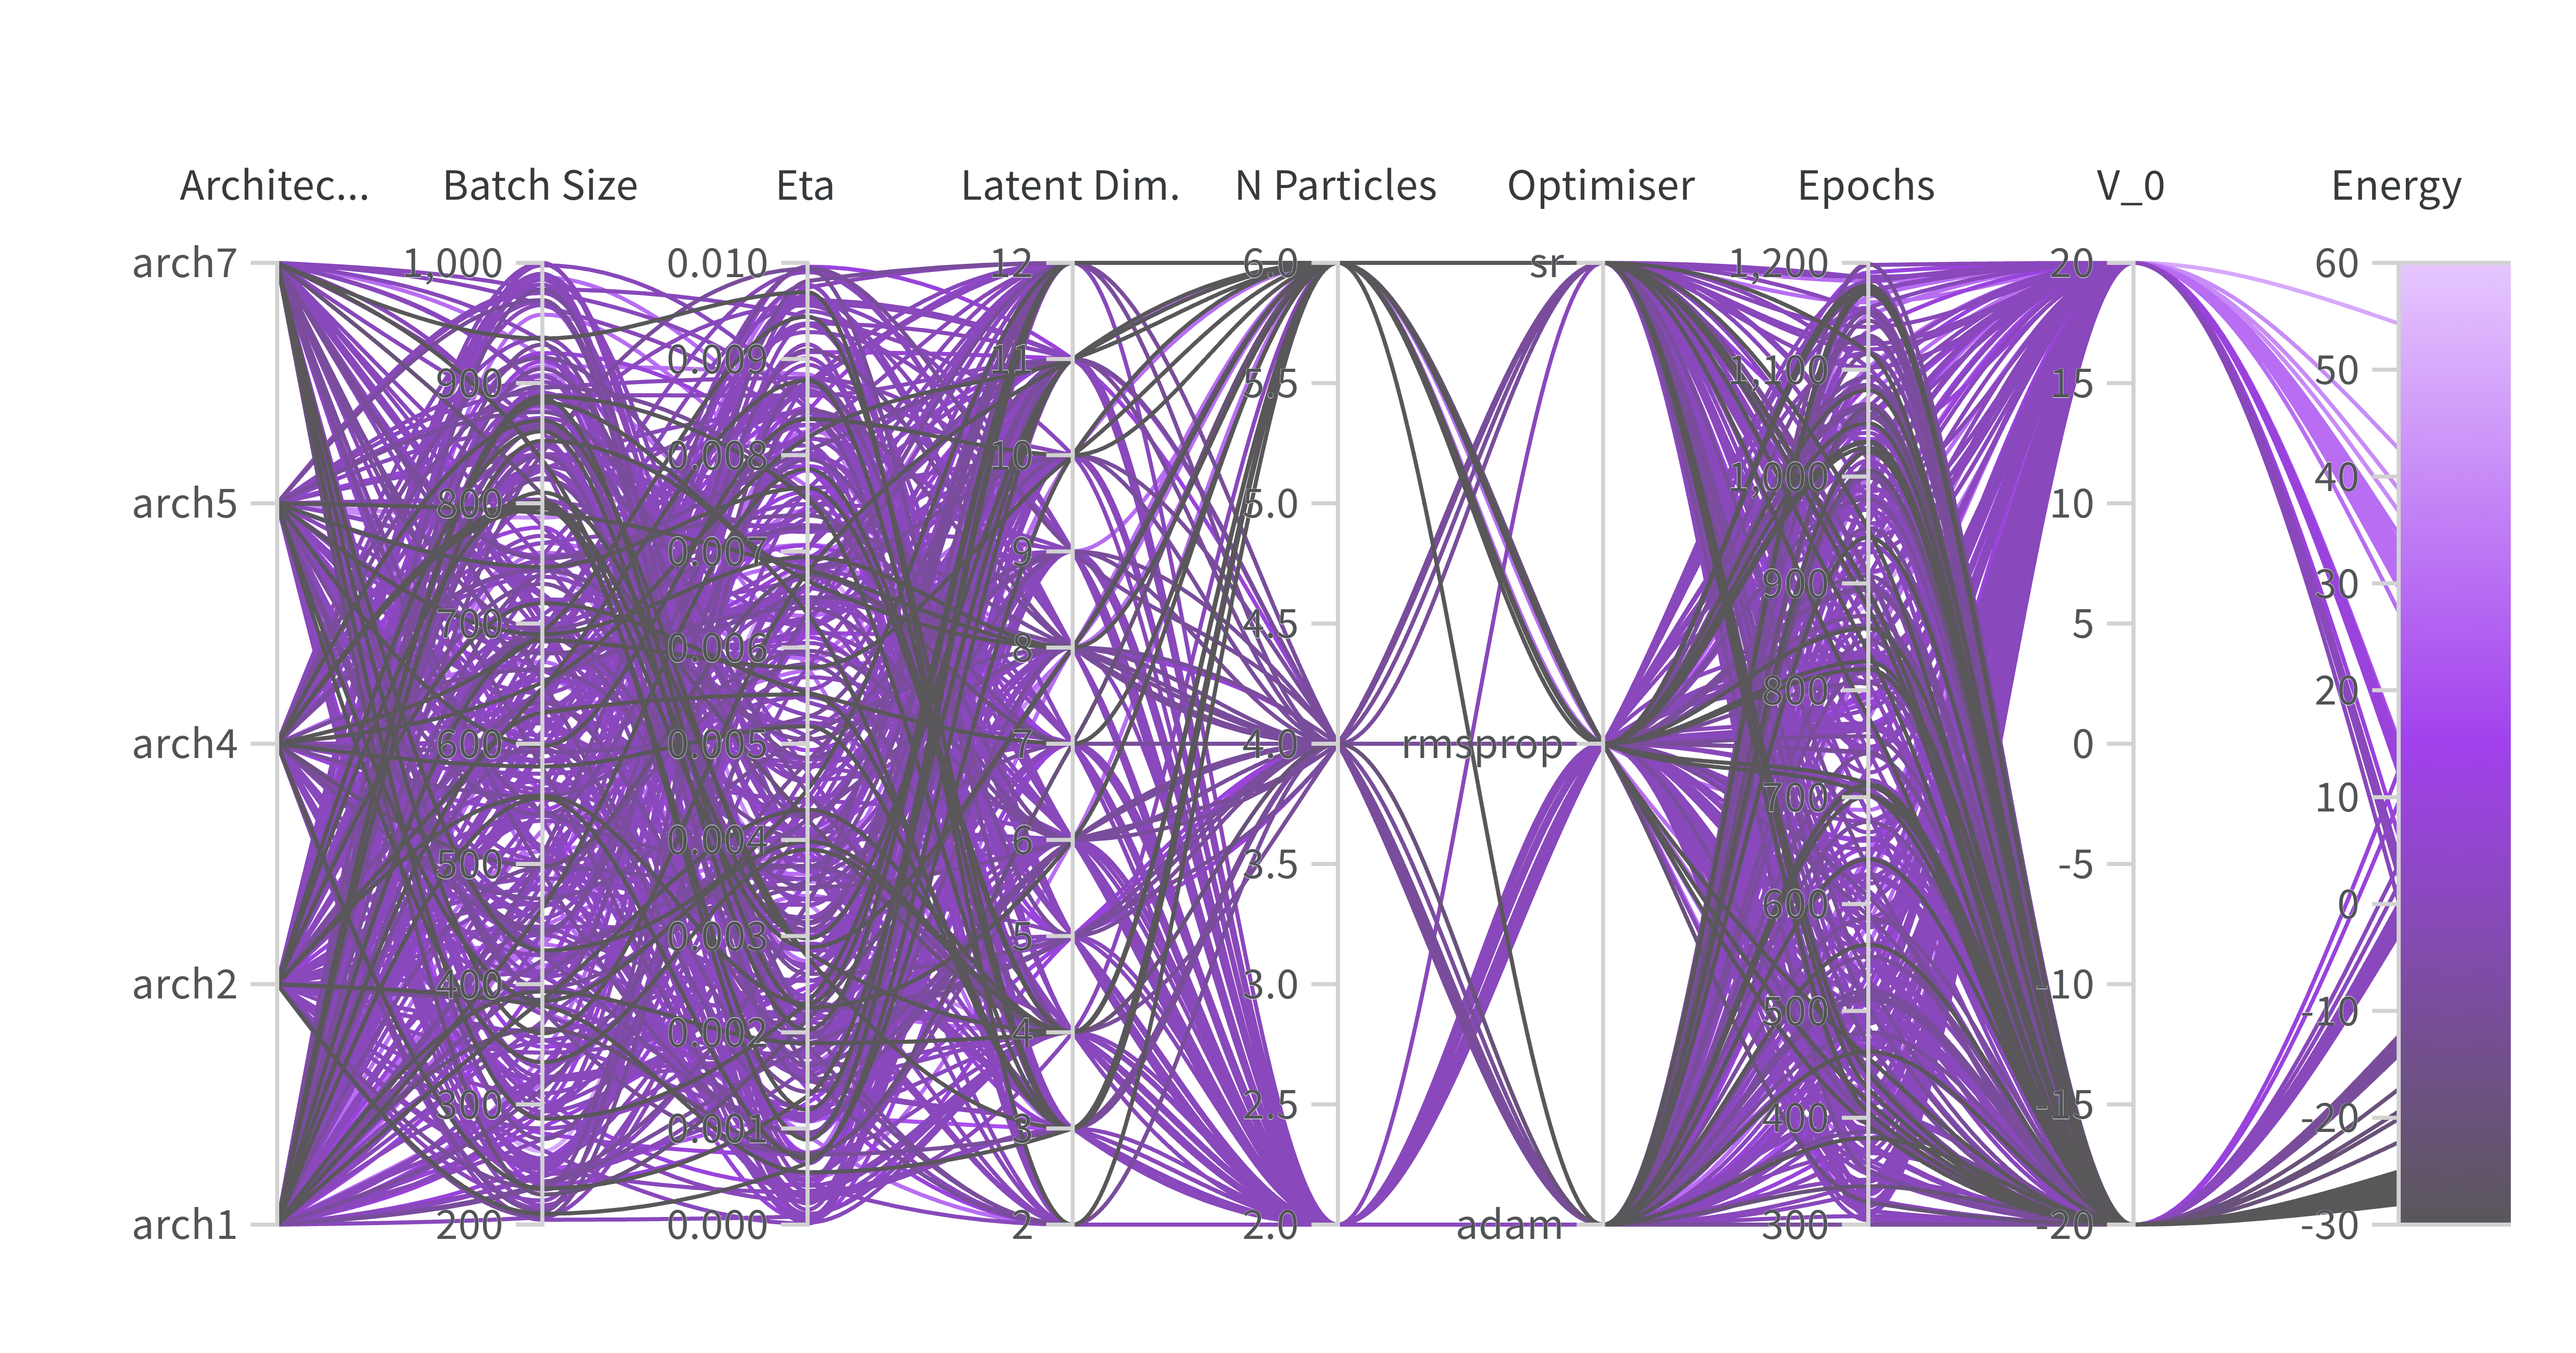
\includegraphics[width=0.8\linewidth]{Chapters/Results/N2/deepset_sweep.png}
    \caption{Sweep over 351 hyperparameters for the standard DSFNN ansatz, from which the results shall be aggregated from. Table \ref{tab:arch} displays the different architectures experimented, here simply marked as ``arch''.}
    \label{fig:ds_complete_sweep}
\end{figure}

\begin{table}[h!]
\centering
\caption{Deep Set architectures Overview for sweep, for the sweep performed in \figref{fig:ds_complete_sweep}. The values missing in the architecture order were discarded for frequent non-convergence behaviour. The latend dimension $L_d$ is chosen independently.}
\label{tab:arch}
\begin{tabular}{@{}lccccc@{}}
\toprule
\textbf{Architecture Nr.} & \multicolumn{2}{c}{\textbf{Activations}} & \multicolumn{3}{c}{\textbf{Layer Sizes}} \\ 
\cmidrule(lr){2-3} \cmidrule(lr){4-6}
 & $\phi$ & $\rho$ & $\phi$ & Pooling & $\rho$ \\ 
\midrule
\textbf{1} & GELU $\times$ 4 & GELU, linear & 7, 5, 3, $L_d$ & Avg & $L_d$, 3, 1 \\ 
\textbf{2} & GELU $\times$ 5 & GELU $\times$ 3, linear & 10, 7, 5, 3, $L_d$ & Avg & $L_d$, 6, 4, 2, 1 \\ 
\textbf{4} & GELU $\times$ 5 & GELU $\times$ 2, linear & 9, 7, 5, 3, $L_d$ & Avg & $L_d$, 5, 3, 1 \\ 
\textbf{5} & GELU $\times$ 5 & GELU $\times$ 2, linear & 14, 9, 7, 5, $L_d$ & Avg & $L_d$, 5, 3, 1 \\ 
\textbf{7} & GELU $\times$ 5 & GELU $\times$ 2, linear & 12, 9, 7, 5, $L_d$ & Avg & $L_d$, 6, 4, 1 \\ 
\bottomrule
\end{tabular}
\end{table}


\subsection{Optimisers}
From the sweep of \figref{fig:ds_complete_sweep}, several results can be aggregated and averages can be taken for certain configurations. For instance, \figref{fig:N2V0=-20_OPT} isolates the case where the interaction strength is $V_0$ and, for a different number of particles, extracts the average energy values for the different choices of optimisers. The figure suggests that among the optimisers evaluated, the stochastic reconfiguration variant consistently outperformed the others, significantly contributing to a lower average value across more than 300 different parameter settings and different number of particles. Although we show only attractive interactions of $V_0 = -20$, the same was observed for repulsive interactions. This motivated the choice of the SR optimiser for all the following results. AdaGrad was consistently the worst optimiser tested, at least for the parameters used.

\begin{figure}[H]
    \centering
    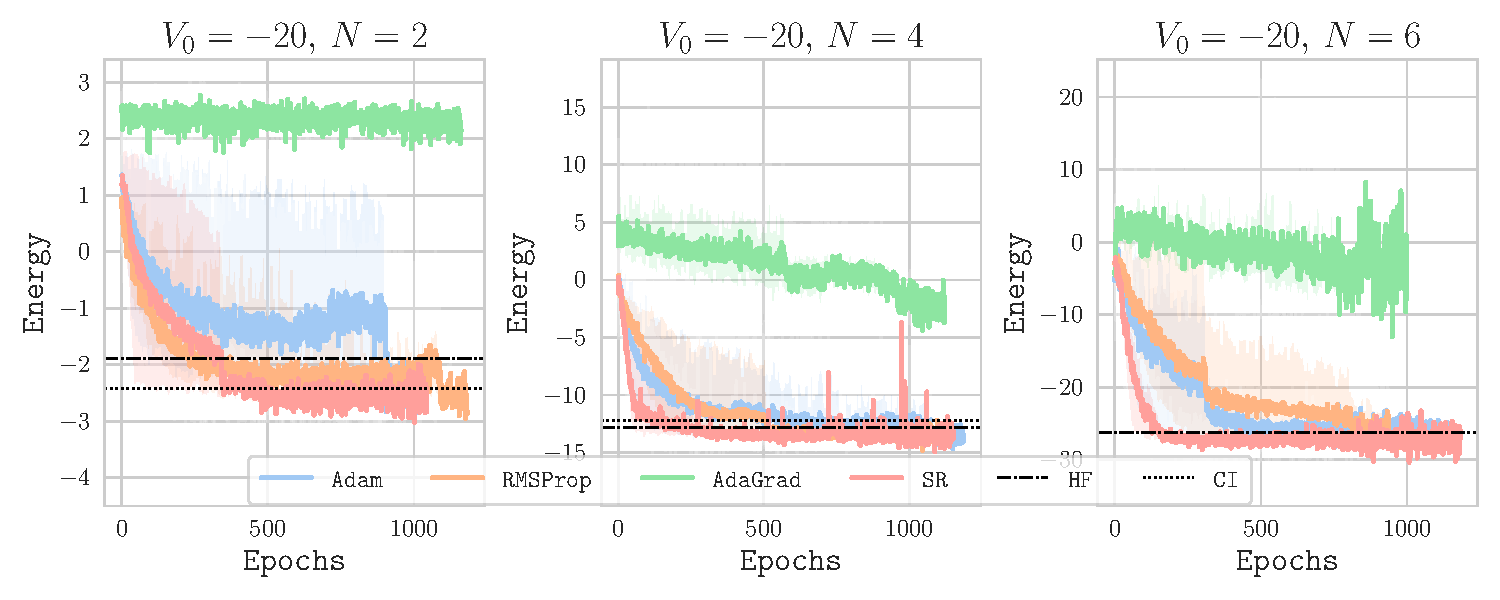
\includegraphics[width=1\linewidth]{Chapters/Results/N2/opti_sweepv0-20.pdf}
    \caption{Training energy averages and standard deviations for the aggregated values of the hyperparameter search of \figref{fig:N2V0=-20_OPT}. Results are displayed for two, four and six particles with interaction $V_0=-20$. Here, the shaded are is not the confidence interval, but the minimum and maximum observed in the parameter search.}
    \label{fig:N2V0=-20_OPT}
\end{figure}

\subsection{Importance sampling}

Another choice that can be investigated from \ref{fig:ds_complete_sweep} is how the expected energy value is affected by the use of importance sampling, discussed in \secref{sec:langevin_imporance}. Figure \ref{fig:comparison_sampling} compares this for different number of particles and the extreme or the interaction strengths, both attractive and repulsive.

\begin{figure}[H]
    \centering
    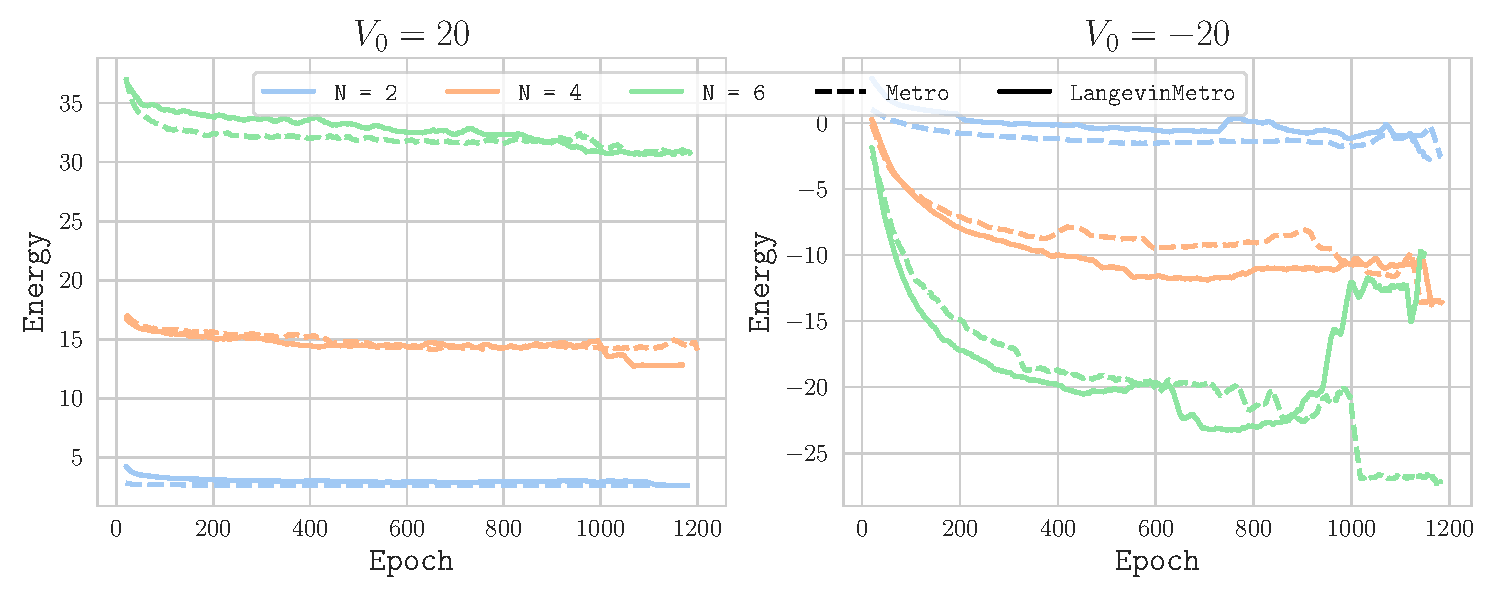
\includegraphics[width=0.9\linewidth]{Chapters/Results/N2/lmh_vs_m.pdf}
    \caption{Comparison of the averaged values over all 321 runs of the sweep shown in figure \figref{fig:ds_complete_sweep} aggregated by number of partciles, interaction stren, rolling window of 20. Errorbars are not included. Here, ``LagevinMetro'' depicts importance sampling.}
    \label{fig:comparison_sampling}
\end{figure}

There is a notable gap regarding whether the choice of importance sampling will, on average, produce better results, as illustrated in \figref{fig:comparison_sampling}. This gap seems to depend on the character of the interaction, where the attractive regime favoured importance sampling over the regular Metropolis algorithm. Although it is challenging to speculate on the exact cause, one potential explanation is the width of the distribution we aim to approximate. In the attractive regime, the distribution tends to be more localised, making standard sampling techniques less efficient. Consequently, for broader distributions, various sampling methods might perform equally well. However, when greater efficiency is needed, importance sampling proved to be more effective.

\begin{figure}[H]
    \centering
    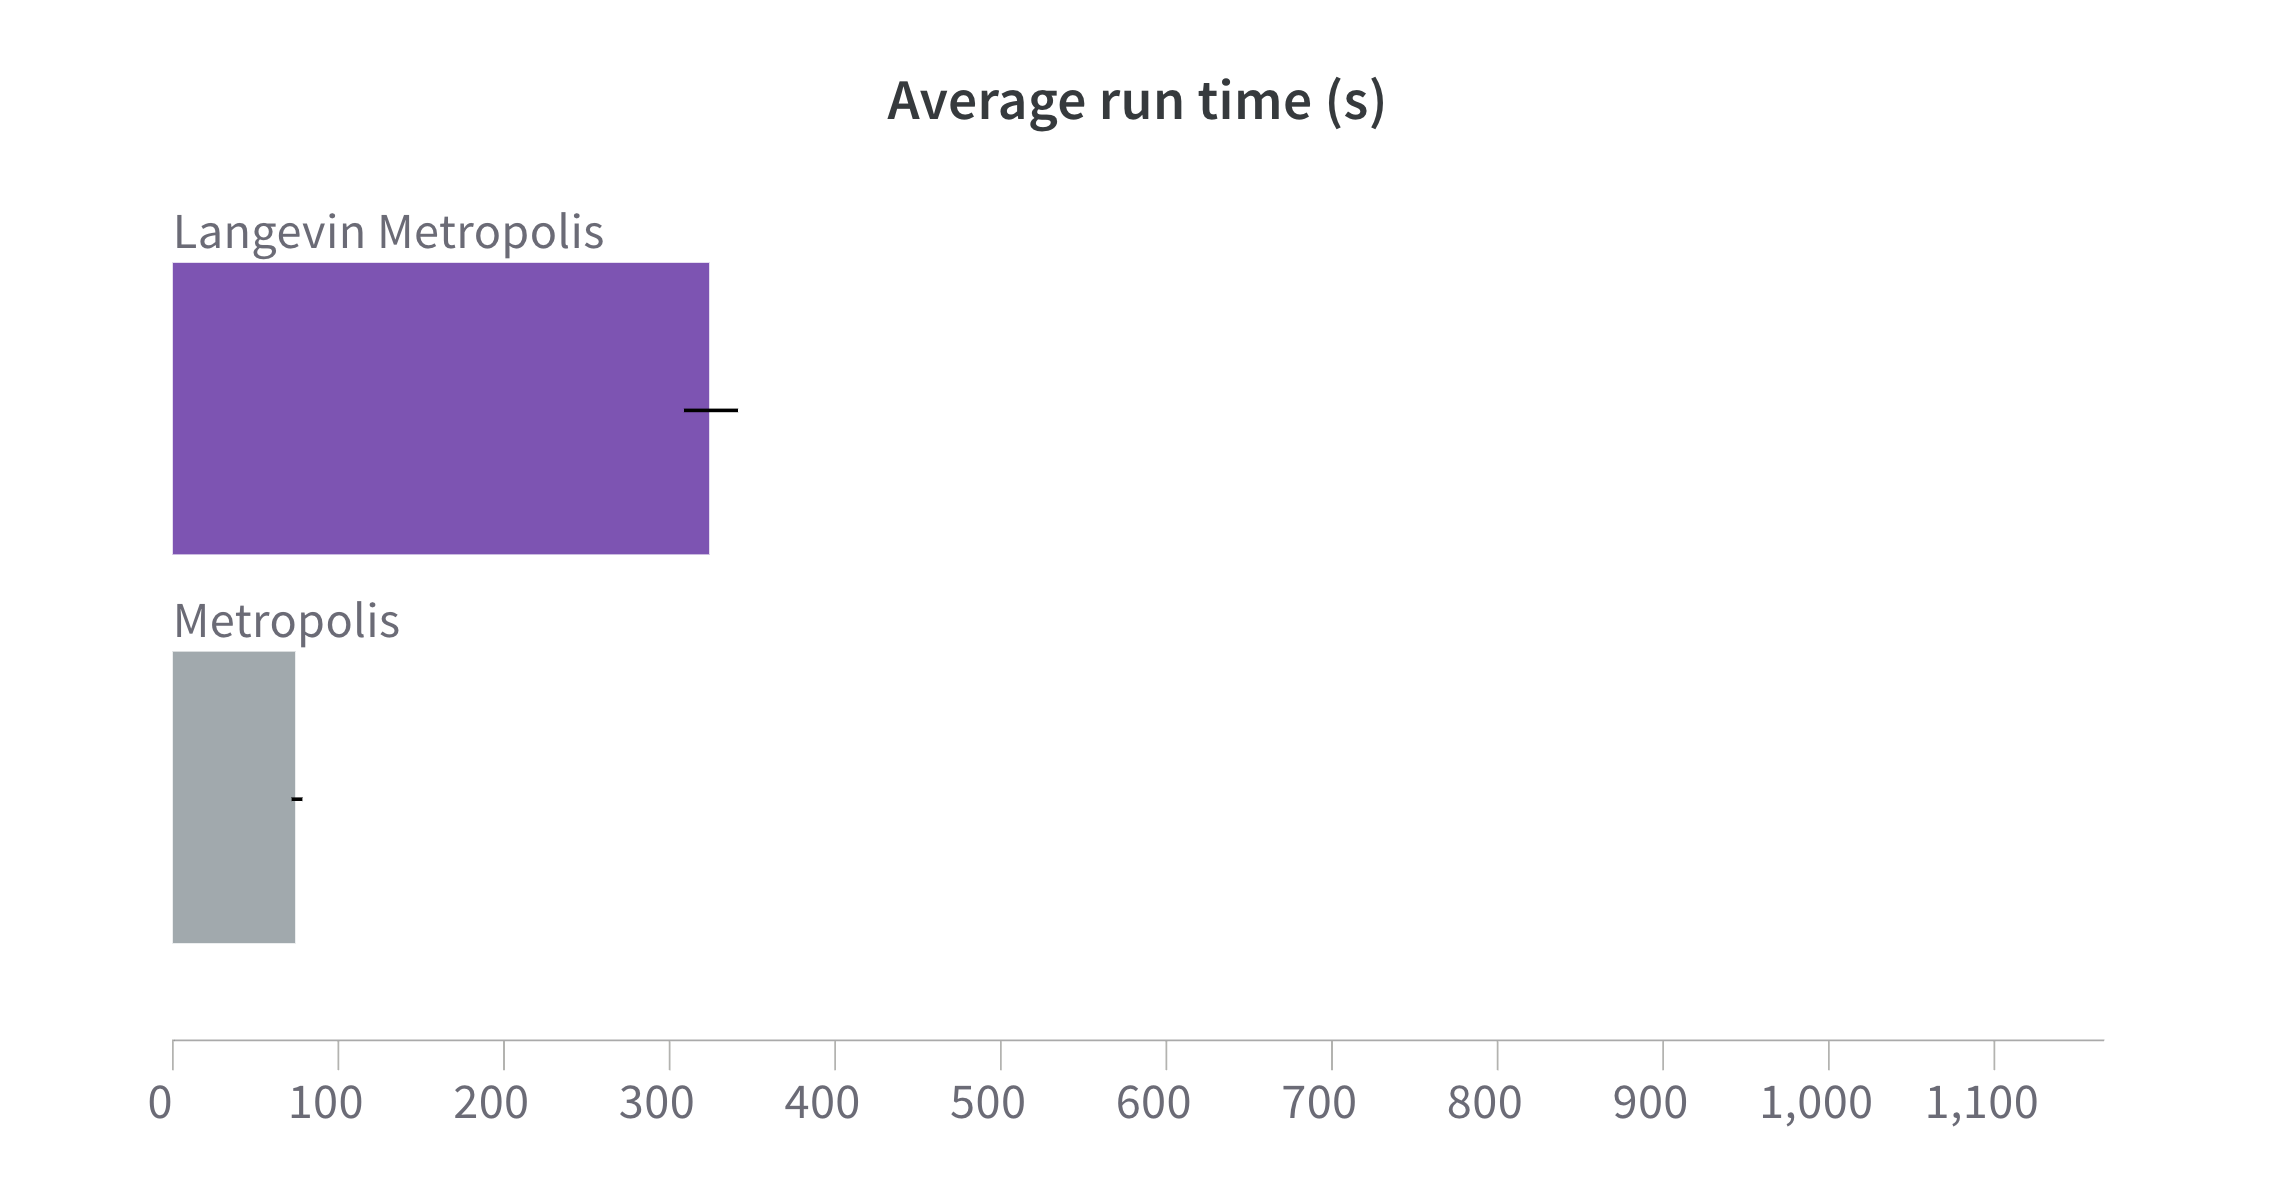
\includegraphics[width=0.7\linewidth]{Chapters/Results/N2/avg_run_time_lm_m.png}
    \caption{Average runtime comparison of the Langevin Metropolis (importance sampling) and the regular Metropolis Makov chain Monte Carlo over 321 randomised runs. The line in black depicts the standard error of the mean.}
    \label{fig:time_metro_langevin}
\end{figure}

Despite the importance sampling technique displaying some advantage over a regular Metropolis Sampling, time complexity must be taken into account. On that note, \figref{fig:time_metro_langevin} shows the average run-time for all configurations displayed in \figref{fig:ds_complete_sweep}. Not all averages include the same batch size or number of training epochs; however, these seem to be equally distributed between sampler options. Figure \ref{fig:ds_complete_sweep} motivates us not to use importance sampling as a method throughout the remainder of this study. There is approximately a threefold discrepancy between average runtimes, and the difference in minimised energy value did not seem to justify its use. The small difference in energy is further supported by \cite{Nordhagen2019}. Although importance sampling has been shown to be necessary for the use of diffusion Monte Carlo \cite{kalos1974helium}, its benefits may not be as significant for VMC.

What explains at least part of the discrepancy in computational time is the need to calculate the drift force, $F = 2\nabla\ln|\psi|$, and the ratio of Green's functions, as displayed in \eqref{eq:met:metric_metropolis_hastings} and \eqref{eq:acceptance_langevin_metro_def}. Although this alone should not have an effect as large as observed, one specific point must be mentioned. For implementation reasons, and to make the Langevin-Metropolis method general to all ansätze, the calculation of the drift force required reshape manipulation of the input position vector. We tried to mitigate this, with no success. As mentioned in \ref{sec:jax}, JAX arrays are supposed to be static, so we strongly believe that a big part of the difference in computational time is due to JAX not being able to fully pre-compile this calculation.

\section{Energy Components}

Now, instead of displaying the average results in a series of configurations, we selected parameters based on the ranges that gave good results from the hyperparameter search of \secref{sec:sweep1d}. For the results that follow, some common choices were made. All results displayed hereafter were performed with trial functions that included a Jastrow factor, and the optimiser of choice was always stochastic reconfiguration. These calculations involve longer training processes and more extensive sampling.

More specifically, \figref{fig:energy_components1d} shows the distribution of the energy components as a function of the interaction strength for all ansätze and different numbers of particles. The different trial functions agreed reasonably well in terms of energy values, and a better comparison can be seen in Table \ref{tab:energy_components1d}.

The energy curves in \figref{fig:energy_components1d} are expected, showing that the energy scale varies with the particle count, while the ratios between the energy components mirror the findings of \cite{drissifermion}, from which we extract some analysis.

First, the total energy $E$ increases when going from an attractive to a repulsive regime. The potential energy increases with the strength of the interaction, but the apparent plateau, together with a decrease in kinetic energy, indicates fermion localisation. This point will be discussed in the analysis of the density profiles. 

When the interaction is extremely attractive, the particles are concentrated in the centre of the trap. In this scenario, the absolute magnitude of the interaction surpasses that of the kinetic energy, and there is almost a cancelation of the trap potential. As also achieved by \cite{drissifermion}, in some instances we observe $\langle K \rangle \leq \langle V_{int} \rangle$, which is a sign of Wigner crystallisation \cite{Vu_2020}.

\begin{figure}[H]
    \centering
        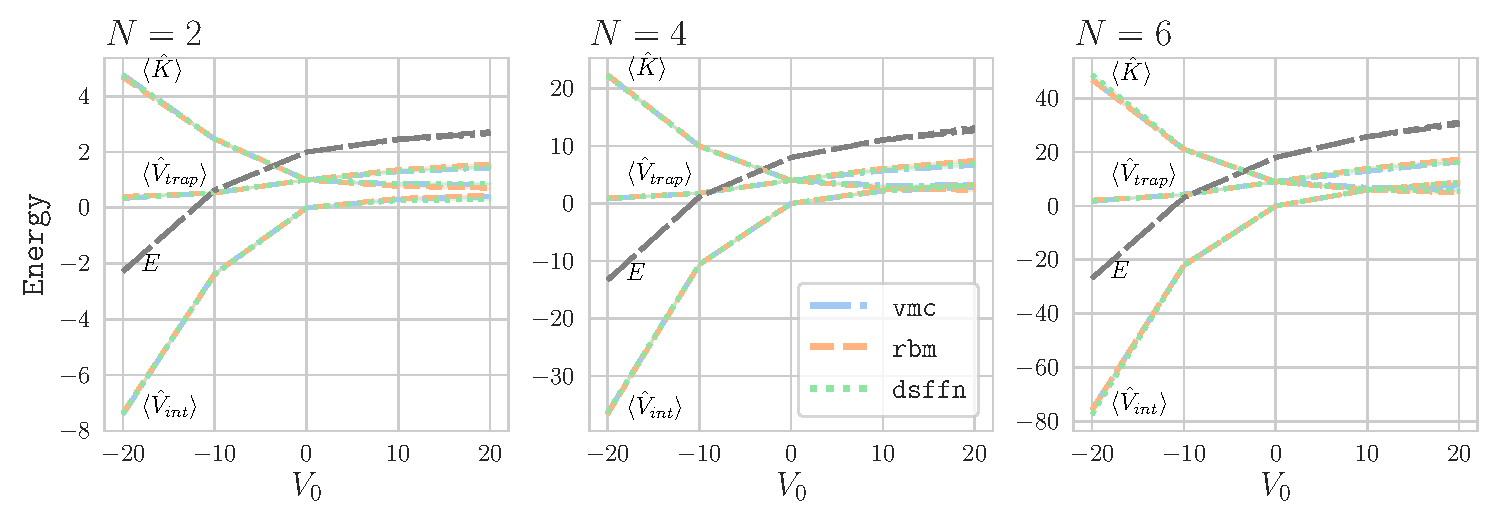
\includegraphics[width=1\linewidth]{Chapters/Results/N2/energy_components_vs_v0.pdf}
    \caption{Energy components as a function of the interaction strength, $V_0$, for different number of particles and trial wavefunctions. All wavefunctions were multiplied by a Jastrow factor. The values were obtained with after $10^{24}$ Monte Carlo samples, SR optimiser and 1500 epochs of training.}
    \label{fig:energy_components1d}
\end{figure}

In Table \ref{tab:energy_components1d} we also show the ratio between kinetic energy and the sum of potential energies for a four-particle system. As dictated by the virial theorem, in the non-interacting case, $\langle E\rangle = 2\langle \hat{K}\rangle = 2\langle \hat{V}_{trap}\rangle$. This is verified with the fraction of the kinetic and potential energies resulting in 1. Again, we note an acceptable yet not perfect agreement between the different models.

\begin{table}[H]
    \centering
\begin{tabular}{c|c|c|c|c|c|c}
\toprule
\multirow{2}{*}{\textbf{Ansatz}} & \multirow{2}{*}{$V_0$} & \multirow{2}{*}{$E$} & \multirow{2}{*}{$\langle \hat{K}\rangle$} & \multirow{2}{*}{$\langle \hat{V}_{trap}\rangle$} & \multirow{2}{*}{$\langle \hat{V}_{int}\rangle$} & \multirow{2}{*}{$\frac{\langle \hat{K} \rangle}{\langle \hat{V}_{trap} \rangle + \langle \hat{V}_{int} \rangle}$} \\
 & & & & & & \\
\midrule
\multirow{5}{*}{DSFFN + SJ}& -20& -13.372(3) & 22.16(1) & 0.8303(5) & -36.364(9) & -0.624
\\
 & -10& 1.1421(9) & 9.941(5) & 1.797(1) & -10.595(4) & -1.130 \\
 & 0& 8.00028(6) & 4.000(2) & 4.000(2) & 0(0) & 1.000 \\
 & 10& 11.009(1) & 2.906(2) & 5.921(2) & 2.182(2) & 0.357 \\
 & 20& 13.244(8) & 3.021(8) & 6.998(3) & 3.224(3) & 0.296 \\
\midrule
\multirow{5}{*}{RBM + SJ} & -20& -13.294(3) & 22.36(1) & 0.9751(8) & -36.63(1) & -0.627 \\
 & -10& 1.145(1) & 9.983(5) & 1.772(1) & -10.610(4) & -1.13 \\
 & 0& 8.00123(8) & 3.998(2) & 4.004(2) & 0(0) & 0.999 \\
 & 10& 11.101(1) & 2.684(1) & 6.089(3) & 2.328(2) & 0.319 \\
 & 20& 13.025(2) & 2.271(1) & 7.476(3) & 3.278(3) & 0.211 \\
\midrule
\multirow{5}{*}{VMC + SJ}& -20 & -13.360(3) & 22.261(9) & 0.8186(4) & -36.439(9) & -0.625 \\
 & -10& 1.1452(9) & 9.978(5) & 1.781(1) & -10.614(4) & -1.130 \\
 & 0& 8.000028(4) & 3.998(2) & 4.002(2) & 0(0) & 0.999 \\
 & 10& 11.0009(7) & 3.161(2) & 5.674(2) & 2.166(2) & 0.403 \\
 & 20& 12.650(1) & 3.222(2) & 6.647(2) & 2.781(3) & 0.321 \\
\bottomrule
\end{tabular}
\caption{A more detailed display of the energy components of \figref{fig:energy_components1d}, for four particles.}
\label{tab:energy_components1d}
\end{table}


\section{One-body Densities}

In terms of one-body density profile, \figref{fig:density_n2} shows in isolation the two-particle case for all ansätze and different interactions, and \figref{fig:densities_all} shows the other cases, up to six particles. From these figures, it becomes clear that, for both an attractive regime and a larger number of particles, getting the models to agree becomes challenging. However, even when the methods disagree, some qualitative points can be addressed. Even for a different number of particles, once the interaction strength is set, the width of the distribution remains the same. Furthermore, the peak of the distributions becomes taller with an increase in the number of particles as $n(\mathbf{x})$ must integrate to $N$, but with the system constrained by the trap.

Importantly, as analysed in terms of energy components, the attractive regime demonstrates a peak at the centre of the trap, in a process corresponding to the bosonization of polarised fermions \cite{valiente2020bose}. On the other extreme, the repulsive interaction results in clear peaks or fringes. The number of peaks corresponds to the number of particles in the system and should, in principle, be symmetric around the origin. 

\begin{figure}[H]
    \centering
    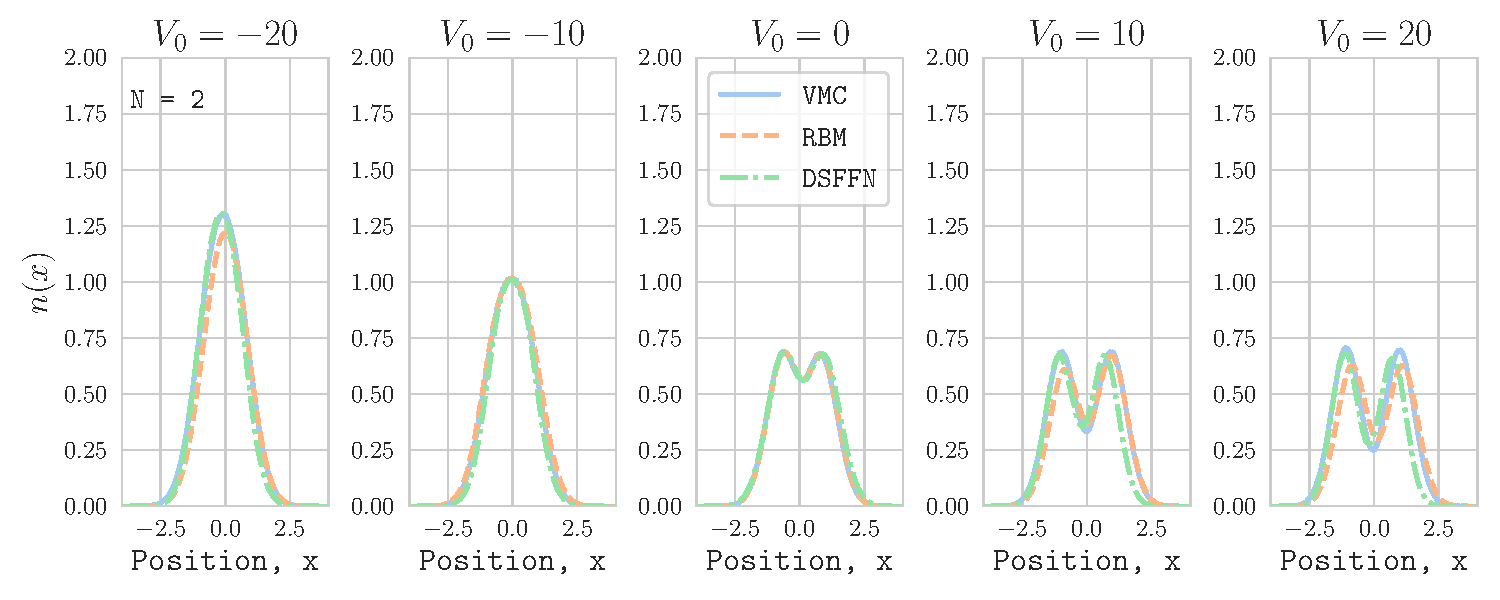
\includegraphics[width=1\linewidth]{Chapters/Results/N2/density_profile_N[2]_nqs_DSFFN.pdf}
    \caption{Density profiles $n(x)$ for two particles at different interaction strengths and for different trial functions, all accompanied by a Jastrow factor. The profile was based on $2^{24}$ samples, with average energies displayed in Tab. \ref{tab:final_energies}}
    \label{fig:density_n2}
\end{figure}

As shown in \figref{fig:densities_all}, the peaks become more pronounced with a stronger interaction, although not all models follow the symmetry constraint well. The VMC function appears to perform the best in this regard. Conversely, the RBM shows significant asymmetry with stronger repulsive interactions and fails to capture the fringes for three interaction strengths in the two-particle scenario. We will explore how this relates to the energy value in \secref{sec:energy}, but we can already discuss this behaviour with respect to the symmetry of the ansätze.

Both mathematically and due to the trap symmetry, the probability density of the antisymmetric wavefunction should be symmetric. Although this seems to be approximately the case in \figref{fig:densities_all} it is certainly not true for all the examples shown. One cause, apart from us not being in the true ground-state, is that the initial ansatz does not perfectly adhere to any symmetry. Due to the potential variations in weights and biases for different particle inputs, the RBM, the VMC Gaussian ansatz, or the Jastrow factor are not ideally symmetric. For instance, even when the Deep Set ensures symmetry and is combined with a determinant that is inherently antisymmetric, the Jastrow factor has the potential to negate this symmetry. We expected this behaviour to be not as dramatic for the Deep Set, but it seems like the VMC was the best in that regard.

\begin{figure}[H]
    \centering
    \begin{subfigure}[b]{0.8\textwidth}
        \centering
        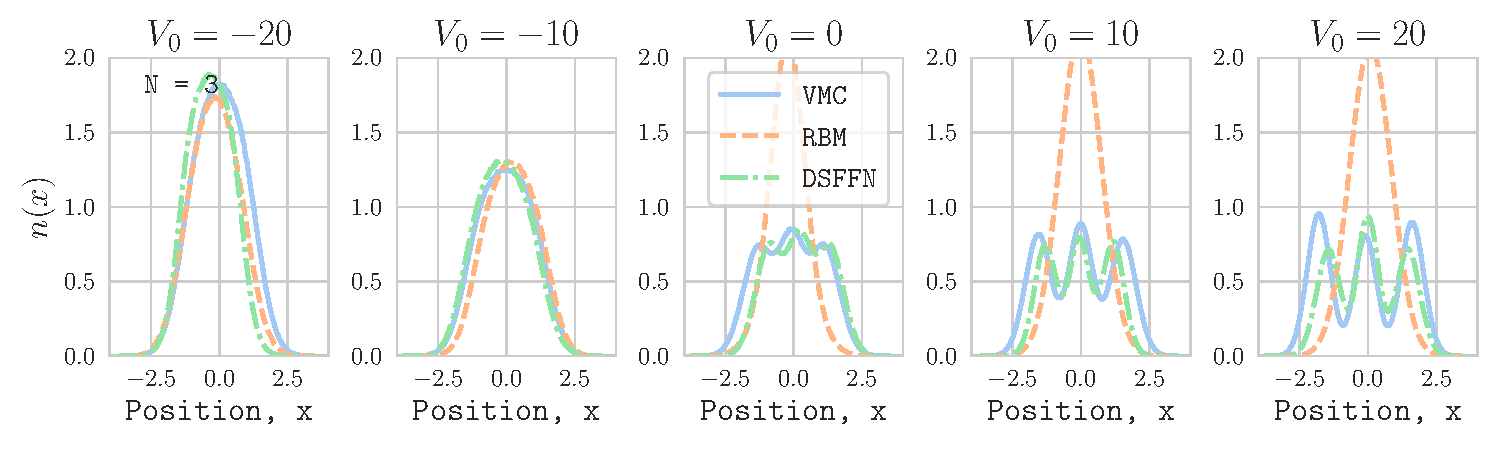
\includegraphics[width=\textwidth]{Chapters/Results/N2/density_profile_N[3]_nqs_DSFFN.pdf}
        \label{fig:total_n2}
        \vspace{-1.25cm}
    \end{subfigure}
    \begin{subfigure}[b]{0.8\textwidth}
        \centering
        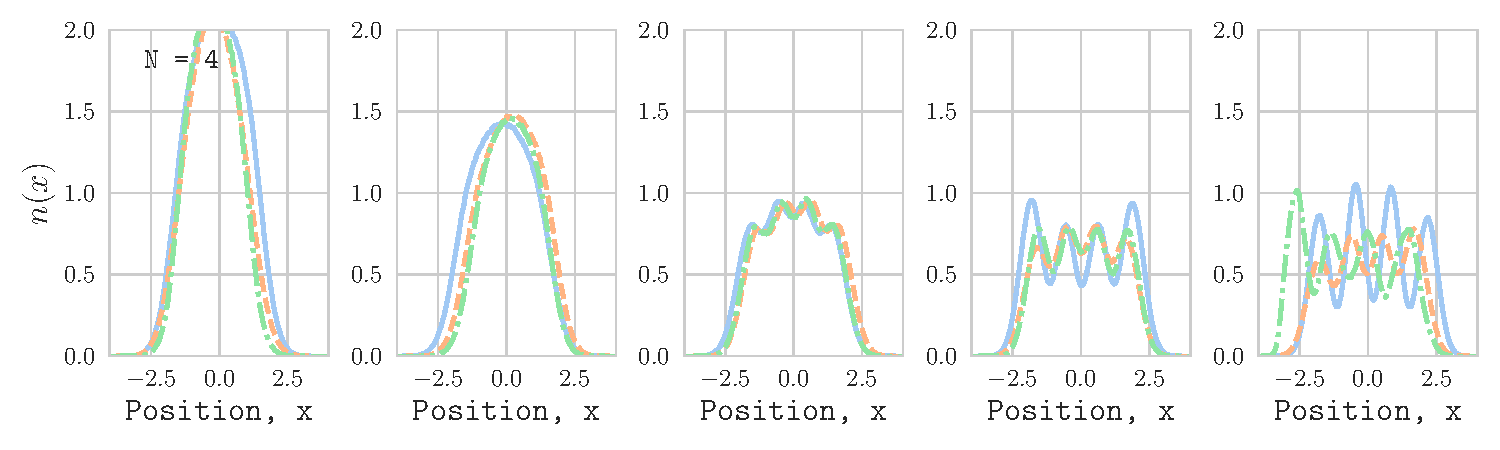
\includegraphics[width=\textwidth]{Chapters/Results/N2/density_profile_N[4]_nqs_DSFFN.pdf}
        \label{fig:total_n4}
        \vspace{-1.25cm}
    \end{subfigure}
    \begin{subfigure}[b]{0.8\textwidth}
        \centering
        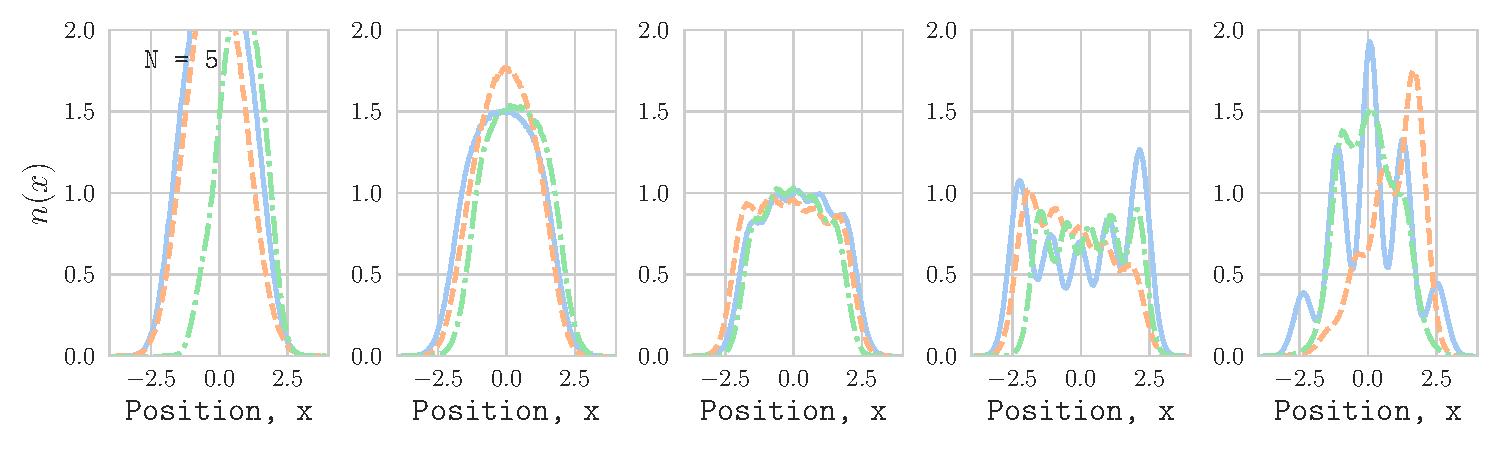
\includegraphics[width=\textwidth]{Chapters/Results/N2/density_profile_N[5]_nqs_DSFFN.pdf}
        \label{fig:total_n6}
        \vspace{-1.25cm}
    \end{subfigure}
    \begin{subfigure}[b]{0.8\textwidth}
    \centering
    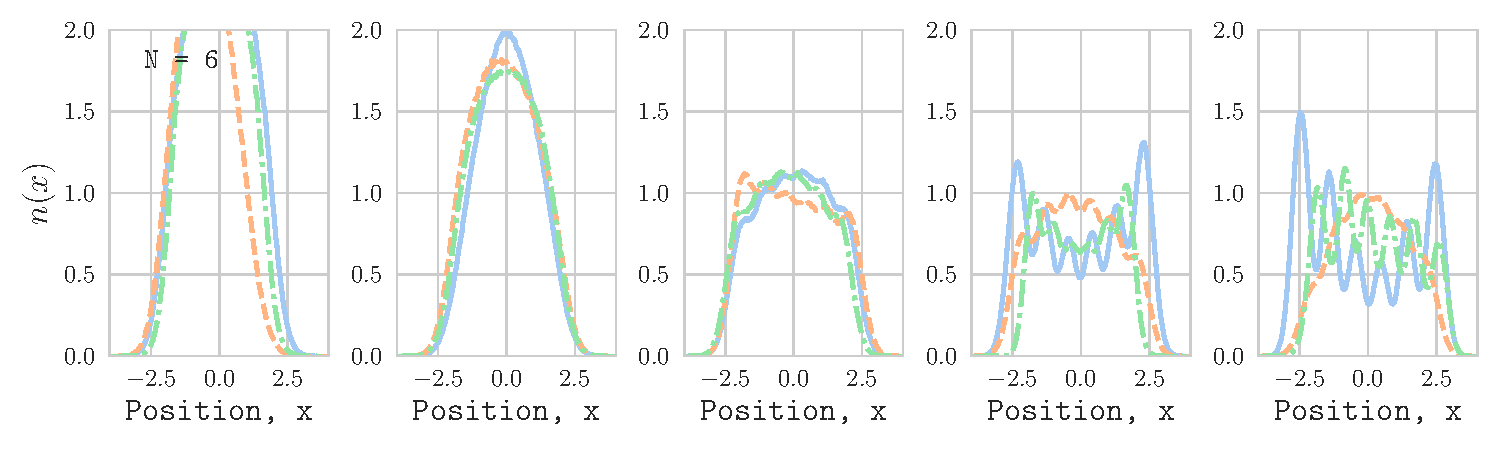
\includegraphics[width=\textwidth]{Chapters/Results/N2/density_profile_N[6]_nqs_DSFFN.pdf}
    \label{fig:total_n6}
    \end{subfigure}
    \caption{Density profiles for different ansätze, after $2^{24}$ MC samples. All ansatze were multiplied by a Jastrow factor, and the sampled energies can be found in Tab. \ref{tab:final_energies}}
    \label{fig:densities_all}
\end{figure}


\section{Overall Energy Comparison}\label{sec:energy}

Figure \ref{fig:corrlation_e} shows that regardless of the model, the energy obtained is lower than the Hartree-Fock energy for every interaction $V_0$. While this figure shows only a two, four and six-particle case, Tab. \ref{tab:final_energies} reveals that this is equally true for other cases. Moreover, there is a clear ease in energy minimisation for the attractive regime. Apart from that, to gauge which models yield the lowest average energy, we can look at the average energy value over all particles and interactions.

\begin{figure}[H]
    \centering
    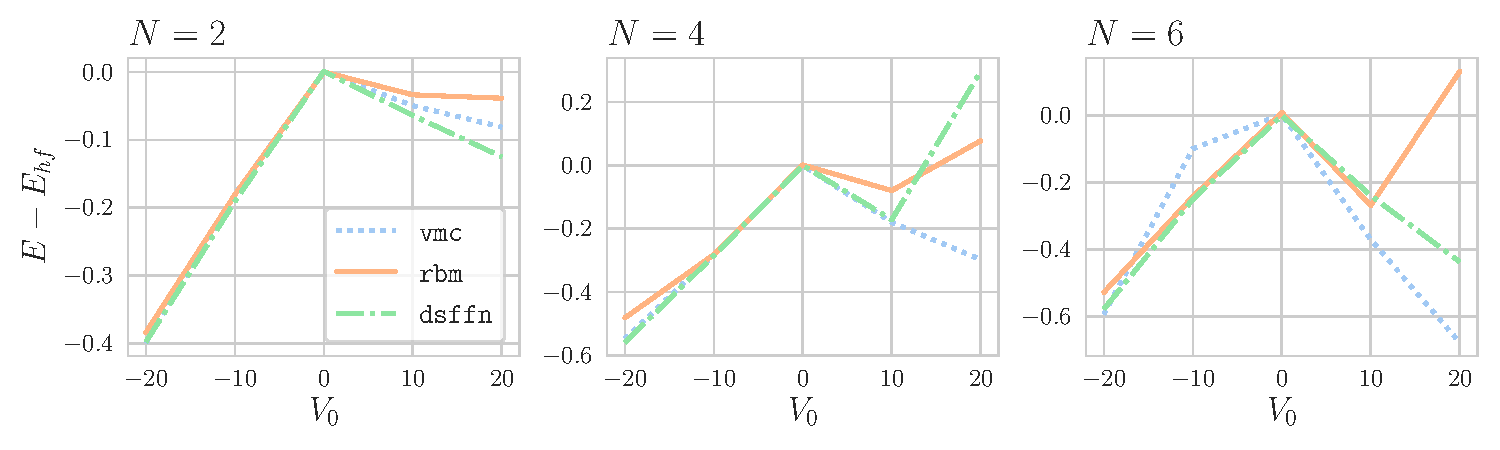
\includegraphics[width=\textwidth]{Chapters/Results/N2//total_energy_vs_v0_n6.pdf}
    \caption{Difference between the energy sampled and the HF energy versus interaction strength $V_0$. Error bars are included but too small to see. For a complete overview of the energies for other number of particles, \ref{tab:final_energies}. All values are result of $10^{24}$ samples after $1500$ epochs of training with Jastrow factor included.}
    \label{fig:corrlation_e}
\end{figure}

We further notice that there is a clear correlation between the lowest energy values obtained in Tab. \ref{tab:final_energies} and a density profile that is closer to what is expected in \ref{fig:densities_all}. For instance, the RBM failed to replicate the expected fringes for three particles in the repulsive interaction. Then, even though the density profile was symmetrical, resembling a Gaussian shape, we see that the energy values for the other two models were lower in that regime. Furthermore, both the RBM and DSFFN model displayed some asymmetry in the five-particle attractive regime, and that is reflected in a significantly higher energy value in comparison to the VMC.

\begin{table}[h]
\centering
\begin{tabular}{c|c|c|c|c|c|c}
\toprule
\textbf{N} & $V_0$& \textbf{DSFFN + SJ} & \textbf{RBM + SJ} & \textbf{VMC + SJ} & \textbf{HF} \cite{drissifermion} & \textbf{CI} \cite{drissifermion} \\
\midrule
\multirow{5}{*}{2} & -20 & -2.289(1) & -2.275(2) & -2.290(1) & -1.891464 & -2.4246 \\
& -10 & 0.6230(5) & 0.6329(6) & 0.6334(6) & 0.813691 & 0.5991 \\
& 0 & 2.00082(5) & 2.000023(7) & 2.0000000(7) & 2.000000 &  \\
& 10 & 2.4401(2) & 2.4705(4) & 2.4545(3) & 2.504193 & 2.4256 \\
& 20 & 2.6396(3) & 2.7258(7) & 2.6832(5) & 2.764479 & 2.6057 \\
\midrule
\multirow{5}{*}{3} & -20 & -7.172(2) & -6.51(2) & -7.249(2) & -6.764263 & -7.0593 \\
& -10 & 0.7709(8) & 1.014(8) & 0.7645(7) & 1.016808 & 0.7300 \\
& 0 & 4.50211(8) & 4.589(2) & 4.500016(6) & 4.500000 &  \\
& 10 & 5.9627(6) & 6.020(1) & 5.9533(4) & 6.061344 & 5.8781 \\
& 20 & 6.760(1) & 6.883(2) & 6.7106(7) & 6.887364 & 6.5153 \\
\midrule
\multirow{5}{*}{4} & 20 & 13.244(8) & 13.025(2) & 12.650(1) & 12.947469 & 12.3408 \\
& 10 & 11.009(1) & 11.101(1) & 11.0009(7) & 11.180564 & 10.8916 \\
& 0 & 8.00028(6) & 8.00123(8) & 8.000028(4) & 8.000001 &  \\
& -10 & 1.1421(9) & 1.145(1) & 1.1452(9) & 1.426522 & 1.1113 \\
& -20 & -13.372(3) & -13.294(3) & -13.360(3) & -12.812753 & -12.1935 \\
\midrule
\multirow{5}{*}{5} & -20 & -19.633(4) & -19.815(5) & -20.065(3) & -19.428348 & -17.3300 \\
& -10 & 1.870(1) & 1.912(1) & 1.923(1) & 2.175499 & 1.8551 \\
& 0 & 12.50157(8) & 12.4975(1) & 12.5004177(5) & 12.5000 &  \\
& 10 & 17.563(1) & 17.645(2) & 17.560(1) & 17.8484 & 17.4648 \\
& 20 & 21.44(1) & 21.033(3) & 20.515(3) & 20.9826 & 20.1357 \\
\midrule
\multirow{5}{*}{6} & -20 & -26.855(4) & -26.805(5) & -26.870(4) & -26.2777 & - \\
& -10 & 3.086(1) & 3.094(2) & 3.237(2) & 3.335750 &  \\
& 0 & 18.00015(4) & 18.0087(2) & 18.0033(1) & 18.0000 &  \\
& 10 & 25.802(3) & 25.773(2) & 25.671(2) & 26.040932 &  \\
& 20 & 30.557(4) & 31.125(5) & 30.316(5) & 30.9932 &  \\
\midrule
\text{Average} & & 4.8237332 & 4.87986612 & 4.7355 & 4.9928 &  \\
\bottomrule
\end{tabular}
\caption{Collection of results for different number of particles, interaction regimes and trial functions. All runs were performed with SR and $2^{24}$ samples, with 1500 epochs of training. All ansätze contained a Jastrow factor. The missing values were not included in the study of reference.}
\label{tab:final_energies}
\end{table}


After discussing the results for the two-dimensional quantum dots, we will offer a broader assessment of the quality of the proposed ansätze and provide possible explanations for the observed differences. For the moment, it is sufficient to highlight the final average energies presented in Tab. \ref{tab:final_energies} indicate that the VMC model performs the best, by a reasonable margin. Behind it is the DSFFN, and last, the RBM. In comparison with the small-basis CI calculations, we observe that in certain cases we can obtain a ground state energy that is lower than theirs. Although this phenomenon is observed in three instances, we focus solely on the validity of the three-particle case with interaction $V_0 = -20$. This selection is due to the small basis CI occasionally showing energy values lower than those from HF calculations. The HF and CI values are sourced from the code provided by \cite{drissifermion}, with the HF equations being solved using integro-differential equations, and this behaviour is not fully understood.


\section{Time Scaling Analysis}\label{sec:time_scaling_1d}

We now discuss how the presented methods scale with the number of particles. In this scenario, a theoretical analysis is a particular challenge. First, not all methods are or should be trained equally. For example, the Deep Set implementation requires a pre-training stage, as described in \ref{sec:pretrain}, where we regress to a Gaussian function. This can be done only once for every architecture and reused for any other problem where the number of particles is the same. For this reason, pre-training timing is not included in the following analysis.

Additionally, the number of parameters in each model is substantially different and that in should change the required number of training steps for convergence. Nevertheless, to make a fair assessment, we show the wall time for three individual training and sampling steps for each ansatz where we consistently used $2^{20} = 1048576$ samples, with 600 training epochs and a batch size of 300 samples. Although the training and batch sizes used here are smaller than those typically used to achieve optimal results, our focus is to illustrate the scaling rather than the absolute values. These averages as a function of the number of particles can be seen in \figref{fig:time_scaling}, where we show measurements for both the SR and Adam optimisers. 

\begin{figure}[H]
    \centering
    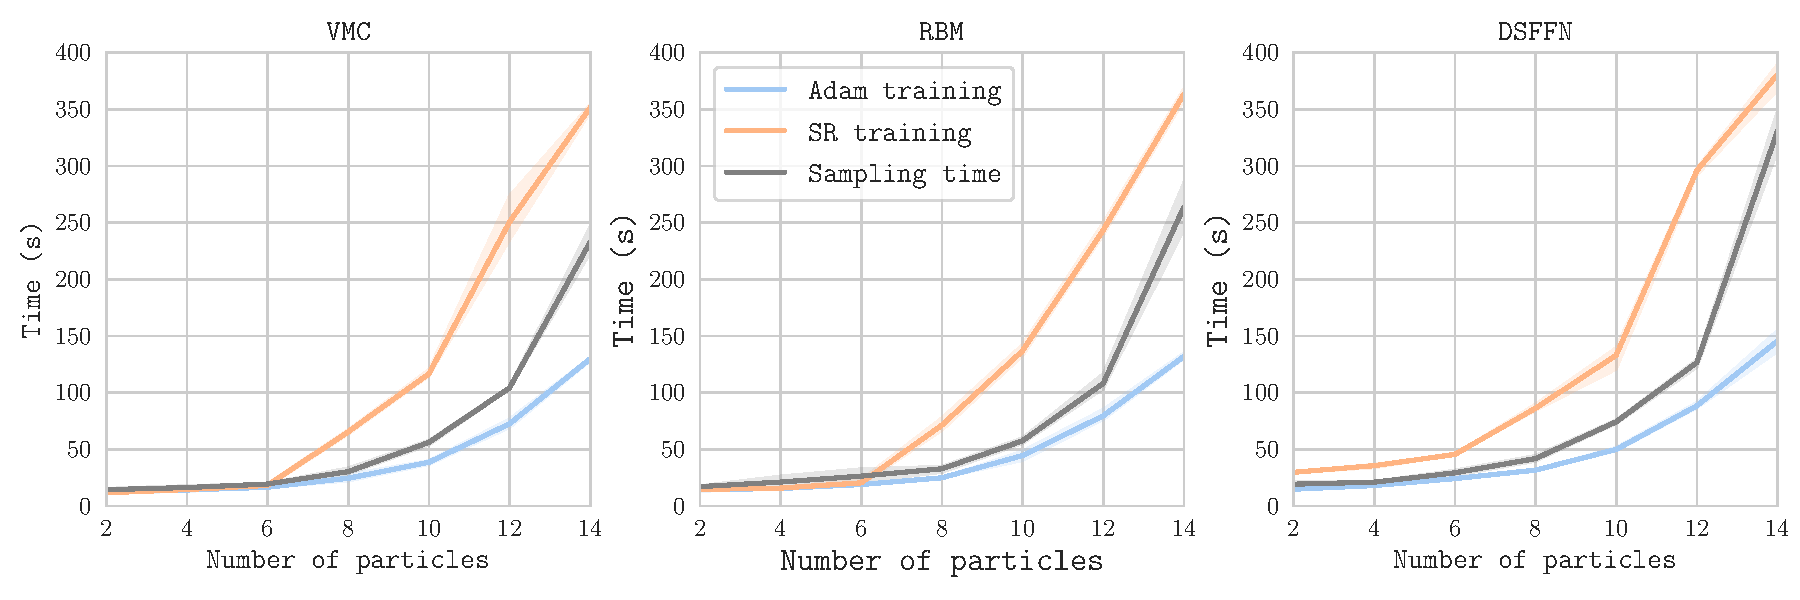
\includegraphics[width=1\linewidth]{Chapters/Results/N2/time_scaling.pdf}
    \caption{Wall time scaling in seconds as a function of number of particles, up to 14 electrons. We display separately the time for sampling and training, where the final wall time is their sum. }
    \label{fig:time_scaling}
\end{figure}

We should also mention that the sampling time does not depend on the optimiser, which is why only one common curve is displayed in \figref{fig:time_scaling}. As expected, the SR method scales worse than Adam, from the costly requirement of inverting the approximate FIM at every epoch, together with the computation of the matrix elements. 

To examine scaling estimations, we present polynomial and exponential fits of the wall time scaling in Tab \ref{tab:time_fits}. Furthermore, for each type of fit, we analyse the effects of constraining the proportionality factor to a constant value, $a = 0.5$. 
The analysis of the unconstrained coefficient reveals that the choice of optimiser, whether for the exponential or polynomial fit, does not significantly affect the order of scaling but rather impacts a constant factor. 

Theoretically, the SR in its brute-force implementation does not scale in the same order as Adam, and it is hard to say if the difference of around $0.5$ for the constrained polynomial fit is expected. While Adam's time complexity is $\mathcal{O}(N_{\theta})$ in time and space, with $N_{\theta}$ the number of parameters, SR involves a matrix inversion time complexity ($\mathcal{O}(N_{\theta}^3)$) and takes $\mathcal{O}(N_{\theta}^2)$ in space. Our block diagonal approximation of the FIM indeed reduces the time and space complexities, but there are still (smaller) matrix inversions in place, as discussed in \secref{sec:kfac}. It might be the case that some precompilation from JAX enables optimisations to take place.

If we accept the polynomial constant of $a = 0.5$, despite a worse $R^2$ score, all the methods follow a polynomial degree scaling between 2 and 3, with DSFFN being the worst and VMC the fastest as expected. A better assessment would surely require us to go beyond the 14 particles used.

Contrary to the DSFFN, the RBM and VMC do not require backpropagation under several compositions of non-linear activation functions. Also, the number of parameters are different. The VMC scales as $N\cdot d$ with particles $N$ and dimensions $d$, while the RBM scales as $N\cdot d \cdot (1 + H) + H$, where $H$ is the number of hidden nodes. For the choice of feed-forward network, the analysis is more complicated as the number of nodes changes for different layers. For timing purposes, we used architecture one from Tab. \ref{tab:arch}, which yielded good results with around $7d + L_d^2 + 8L_d +68$ parameters, where $L_d$ is the size of the latent dimension, often between four and ten.

\begin{table}[H]
    \centering
    \caption{Polynomial and exponential fits of time scaling vs. Number of Particles. The leftmost fits do not constrain any coefficients, while the leftmost fits constrains $a = 0.5$.}
    \begin{tabular}{llcccccc|cccc}
        \toprule
        \label{tab:time_fits}
        \textbf{Ansatz} & \textbf{Opt.} & \multicolumn{3}{c}{\textbf{Poly.} $(aN^b)$} & \multicolumn{3}{c}{\textbf{Exp.} $(ae^ {Nb})$} & \multicolumn{2}{c}{\textbf{Poly.} $(0.5N^b)$} & \multicolumn{2}{c}{\textbf{Exp.} $(0.5e^ {Nb})$} \\
        \cmidrule(lr){3-5} \cmidrule(lr){6-8} \cmidrule(lr){9-10} \cmidrule(lr){11-12}
        & & \textbf{a} & \textbf{b} & \textbf{R\textsuperscript{2}} & \textbf{a} & \textbf{b} & \textbf{R\textsuperscript{2}} & \textbf{b} & \textbf{R\textsuperscript{2}} & \textbf{b} & \textbf{R\textsuperscript{2}} \\
        \midrule
        \multirow{2}{*}{VMC} & Adam & 0.03 & 3.15 & 0.96 & 2.89 & 0.27 & 0.99 & 2.05 & 0.91 & 0.40 & 0.92 \\
         & SR & 0.13 & 3.01 & 0.99 & 8.09 & 0.27 & 0.98 & 2.48 & 0.97 & 0.48 & 0.84 \\
        \midrule
        \multirow{2}{*}{RBM} & Adam & 0.07 & 2.85 & 0.96 & 3.93& 0.25 & 0.99 & 2.07 & 0.93 & 0.40 & 0.88 \\
         & SR & 0.18 & 2.90 & 1.00 & 9.14 & 0.27 & 0.99 & 2.49 & 0.99 & 0.48 & 0.83 \\
        \midrule
        \multirow{2}{*}{DSFFN} & Adam & 0.17 & 2.53 & 0.93 & 5.29 & 0.24 & 0.98 & 2.10 & 0.92 & 0.41 & 0.79 \\
         & SR & 0.43 & 2.59 & 0.97 & 14.37 & 0.24 & 0.97 & 2.52 & 0.97 & 0.48 & 0.73 \\
        \bottomrule
    \end{tabular}
\end{table}
